\subsection{Unimodal Functions}

By unimodal function, we mean one of two behaviors of the function:

\begin{itemize}
  \item The function strictly increases first, reaches a maximum (at a single point or over an interval), and then strictly decreases.
  \item The function strictly decreases first, reaches a minimum, and then strictly increases.
\end{itemize}

\begin{figure}[ht]
    \centering
    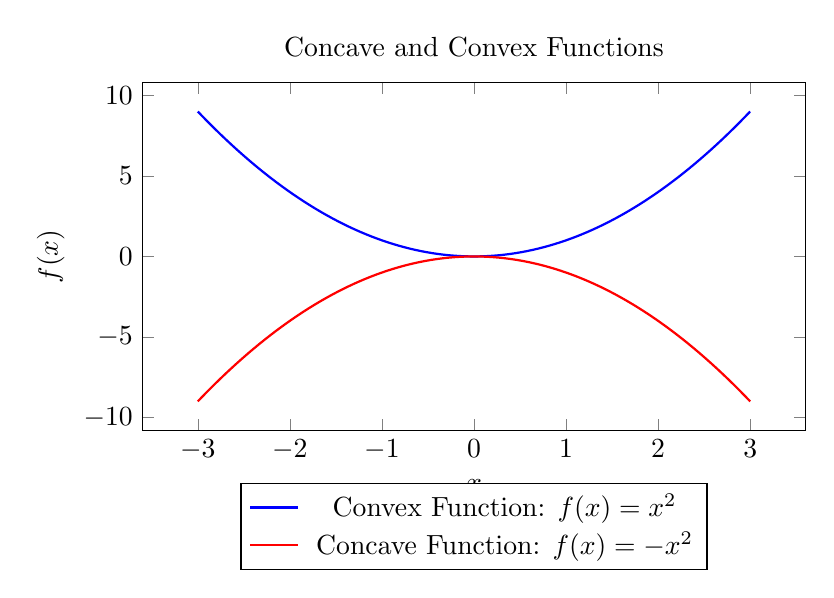
\begin{tikzpicture}
        \begin{axis}[
            title={Concave and Convex Functions},
            xlabel={$x$},
            ylabel={$f(x)$},
            domain=-3:3,
            samples=100,
            width=10cm,
            height=6cm,
            legend style={
              at={(0.5,-0.15)}, % Position legend below the plot
              anchor=north,     % Anchor legend at the north (top) edge
              legend columns=1, % Arrange legends in 2 columns
              column sep=1ex    % Space between columns
            }
        ]
        
        % Convex function (upward parabola)
        \addplot [
            color=blue,
            thick
        ]
        {x^2};
        \addlegendentry{Convex Function: $f(x) = x^2$}

        % Concave function (downward parabola)
        \addplot [
            color=red,
            thick,
        ]
        {-x^2};
        \addlegendentry{Concave Function: $f(x) = -x^2$}
        
        \end{axis}
    \end{tikzpicture}
    %\caption{A convex function (upward parabola) and a concave function (downward parabola).}
\end{figure}

